\section{Introduction}

\subsection{Présentation du projet}
Le COPEVUE a lancé un appel d'offre dans le cadre de la réalisation d'un système de monitoring de sites isolés. Il s'agit donc de concevoir en premier lieu une solution technique permettant de répondre au mieux aux exigences fonctionnelles et non fonctionnelles que le COPEVUE formule. De façon synthétique notre équipe va proposer une solution permettant de surveiller des sites naturels difficiles d'accès (souvent à cause des conditions environnementales) et peu peuplés. Dans ces sites isolés sont souvent regroupés des postes de travail et ces zones doivent pouvoir être surveillées en dépit de la distance qui les sépare du bureau de contrôle.
% On reprend ce qui a déjà été fait dans les autres documents.

\subsection{Présentation du document}

Ce dossier présentent les besoins nécessaires par rapport à la solution d'acquisition des données des capteurs, et de la transmission de celles-ci avec la base de la station. Nous essayerons tout d'abord de voir quels sont les objectifs de cette solution technique, les utilisateurs concernés et les problèmes pouvant se présenter, autant dans son développement, sa mise en oeuvre, et enfin sa maintenance. Ce document est accompagné d'annexes permettant d'appronfondir certains sujets plus techniques sur lesquels nous n'avons pas voulu nous attarder dans un but de clarté.

\subsection{Documents applicables / Documents de référence}

% Décider ensemble de ce que l'on met dans ce genre de sections.

\subsection{Terminologie et abréviations}

% A complêter au fur et à mesure.
\begin{itemize}
\item Base (de la station) : système informatique équipé d'un OS linux permettant de communiquer avec les capteurs et le serveur central. La base peut aussi enregistrer quelques données et permet de configurer la plupart des éléments de la station.
\item Mode sommeil : mode dans lequel le microcontroleur et le capteur ne consomme que très peu d'énergie. Aucune acquisition et aucun calcul ne doivent être fait pendant cette periode. Le micro-controleur attend d'être réveillé par un évenement materiel ou logiciel.
\end{itemize}

\section{Présentation du problème}

\subsection{Buts, nature du logiciel, utilisateurs concernés}

Le logicel qui doit être implementé a deux fonctions:
\begin{itemize}
\item L'acquisition des données des capteurs à un intervalle de temps définie préalablement,
\item L'envoi de ses données à la base de la station à un intervalle de temps régulier. Pendant cette connexion, la configuration des capteurs par la base devra être possible. Ainsi, l'écart entre chaque acquisition ou transmission devra être parametrable. Cette configuration sera faite pendant la transmission avec la base.
\end{itemize}

Ce composant logiciel devra ainsi intéragir avec la base de la station, lui envoyer les données et vérifier si une reconfiguration est necessaire. Il devra également se charger de récuperer la valeur du capteur auquel il est attaché. Ce composant logiciel devra impérativement être économes et devra passer la grande majorité du temps en mode "sommeil".

D'un point de vue plus technique, ce logiciel devra s'exécuter sur un controleur attaché à une puce ZigBee, au capteur et à la batterie longue durée.

Le protocole de communication utilisé par les modules de transmission avec la base sera décrit plus loin dans ce document.

Ce document va aussi porter sur le matériel exploité par le logiciel précédement cité, à savoir le module de communication ZigBee. Les attentes par rapport à celui-ci seront également décrite.

\subsection{Formulation des besoins, exploitation et ergonomie, expérience}

Le système présentement présenté doit répondre à deux besoins bien distincts, et ce quelque soit la localisation géographique du système dans le monde :

\parapraph{Acquisition} Le système doit pouvoir recuperer la valeur des capteurs de la façon suivante :

\begin{itemize}
\item Le micro-controlleur sera reveillé selon la periode d'acquisition, il relevera la valeur du capteur 
\item Selon la configuration de la periode de transmission, soit la donnée du capteur est en enregistré temporairement, soit directement envoyé à la base
\item Le micro-controlleur devra s'adapter au capteur pour pouvoir gerer les differents types d'acquisitions
\item Si besoin, le niveau de la batterie doit également être verifié
\item Le module doit être capable de se reconnecter à la base en cas de déconnexion
\item En cas de situation critique (batterie ou capteur), les données necessaire à l'analyse de cette état devront être transmis à la base le plus tôt possible
\end{itemize}

\paragraph{Transmission} Pendant la transmission, le système doit être capable d'analyser les données et d'envoyer les informations suivantes à la base :

\begin{itemize}
\item Les informations nécessaire du capteur
\item Au besoin et en cas de situation critique, le niveau restant de la batterie doit être envoyé
\item La date du prochain reveil et eventuellement les informations utiles du micro-controlleur
\end{itemize}

Pendant la transmission, le système doit être capable de recevoir des données correspondant à la reconfiguration du module :

\begin{itemize}
\item Les différents quantum de temps définissant la granularité avec laquelle le système transmet les résultats a la base, en analysant les données des capteurs.
\item La configuration du capteur doit être possible.
\end{itemize}

Voici un schéma resumant les différents composants du module d'acquisition :

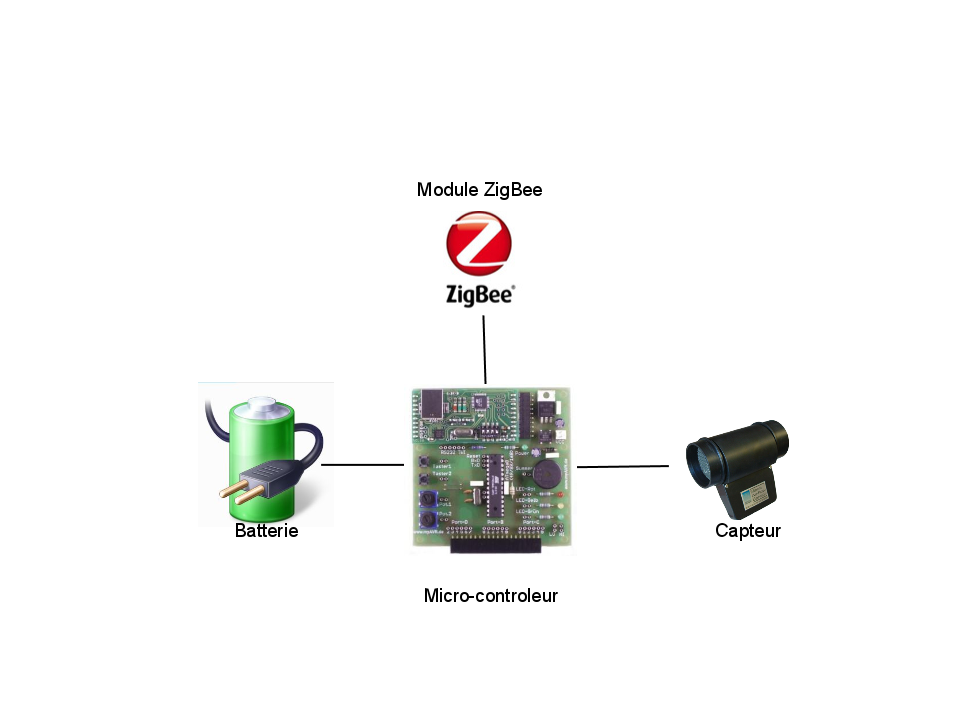
\includegraphics[width=15cm]{schemacdc.png}

\subsection{Portée, développement, mise en oeuvre, organisation de la maintenance}

L'application devra être programmé en utilisant le langage C. Des tests unitaires et fonctionnels devront être implémenté.

Les differents éléments (programme et tests) seront documentés, afin de faciliter la maintenance du système et de permettre des futures améliorations. Cette documentation devra contenir les différentes difficultés et erreurs rencontrées lors de la phase de developpement.

\subsection{Limites}

Le logiciel devra se limiter aux fonctions décrites dans ce documents. L'autonomie, la simplicité et la fiabilité du système sont primordiales. Toute fonctionnalité non décrite sera inutile.

\section{Exigences fonctionnelles}
\subsection{Fonctions de base, performances et aptitudes}

Le module d'acquisition doit sortir du mode "sommeil" à un intervalle de temps régulier définie en configuration. Le système doit rester le moins de temps possible en mode "éveillé" pour respecter les contraintes d'autonomie.
L'acquisition du capteurs se fera via une interface. L'implémentation de cette interface ne doit pas être programmé et fera l'affaire d'une autre étude. Cette interface, réspecté par tous les types de capteurs, sera décrites plus loin.

L'acquisition de la batterie devra être effectué régulierement à un intervalle de temps définie par la configuration. Une interface similaire à celle du capteur sera utilisé pour reperer le niveau de batterie.

Après l'acquisition, une tentative de connexion devra être effecté avec la base de la station. Si celle-ci reussi, les données des capteurs et de la batterie sont transmises. Sinon, elles sont stockées temporairement. Ce stockage doit être étudié précisement et ne doit par être effectué si la consommation devient trop importante. Les données seront dans conservé dans les cas où la situation est critique.  

Pendant la transmission, la configuration doit être possible. Les points suivants peuvent être modifié :
\begin{itemize}
\item La valeur du capteur en cas de mauvais reglage de celui ci,
\item La periode d'acquisition des données du capteur,
\item La periode d'acquisition des données de la batterie,
\item La periode de transmission, dans la plupart des cas cette periode sera égal à la periode d'acquisition des données du capteur. 
\end{itemize}

\subsection{Contraintes d'utilisation}

Le système ne doit pas pouvoir être utilisé par un utilisateur humain. La sécurisation des données envoyées est à prévoir, il ne faut pas qu'un utilisateur externe puissent intercepter les données ou interagir avec le systeme. Cette interaction pourrait mener à des disfonctionnements du système. Un système de cryptage, tel qu'un certificat, ou une autre méthode de sécurisation doit être mis en place.
Il faut prévoir qu'une opération de maintenance sur site a un coût élevé, le système doit être réflechit pour limiter au maximum les disfonctionnements necesitant un déplacement. 

\subsection{Critères d'appréciation de la réalisation effective de la fonction}
Les différents critères seront pris en compte pour juger le système. A ces critères sont ajoutés la nécessité et le taux de difficulté estimé. Ces valeurs vont de 0 à 10, 0 étant la valeur la plus basse :

\begin{tabular}{|l|l|l|}
  \hline
  Critère & Nécessité & Difficulté \\
  \hline
  Sécurisation du protocole de transfert & 7 & 6 \\
  Dépense énergetique & 9 & 5 \\
  Stabilité & 9 & 7 \\
  Facilité de la maintenance du code & 8 & 4 \\
  Clarté de la documentation  & 8 & 4 \\
  \hline
\end{tabular}

\section{Exigences non fonctionnelles}

\section{Contraintes imposées, faisabilité technologique, moyens}
\subsection{Sûreté, planning, organinsation, communication}
Le protocole utilisé est le ZigBee, qui à l'avantage d'être simple d'utilisation. Cependant, il est necessaire de prévoir un temps d'apprentisage de cette technologie si necessaire. 

La communication avec la maitrise d'ouvrage peut être envisagé et sera si necessaire organisé par la maitrise d'oeuvre. Le planning devra également prendre en compte une période de test.

Voici le planning prévisionnel du projet :

\begin{tabular}{|l|l|}
  \hline
  Phase & Durée prévisionnelle \\
  \hline
  Spécification Code et Tests & 1 mois \\
  Dévellopement Code et Tests & 3 mois \\
  Tests intégration avec le système entier & 2 mois \\
  Finalisation et reprise des élements  & 2 mois \\
  \hline
  Total  & 8 mois \\
  \hline
\end{tabular}

\subsection{Complexité}
Le système envisagé ne demande pas une complexité importante. Le protocole ZigBee étant largement documenté, le reste du système reste simple. Le fonctionnement de ce module avec le reste du sytème doit être pris en compte. 
La principale difficulté reste la stabilité du système, celui ci doit absolument être fiable. 

\subsection{Compétences, moyens et règles}
Les compétences techniques suivantes sont exigées :
\begin{itemize}
\item Expertise en système embarquée
\item Programmation bas niveau
\item Connaissance de protocole reseau
\item Securisation reseau
\end{itemize}
Ce projet nécessite peu de ressource materiel, l'équipe devra être équipé de technologie pour programmer et debuguer la carte choisi. 

\section{Configuration cible}

\subsection{Matériels et logiciels}
Le materiel utilisé pour dévelloper le module est le suivant:

Pour le controleur qui à la responsabilité de gérer le capteur, le ZigBee et le niveau de batterie, il a été decidé d'utiliser un carte FOX Board LX832.

Pour le ZigBee, un carte de type EB051 sera utilisé, la puce ZigBee est directement intégré au circuit de la carte. Cette carte permet une utilisation simplifié des protocoles ZigBee.
Si le capteur n'en est pas doté, un micro-controleur sera couplé au capteur. Ce cahier des charges ne prends pas en compte cette partie. Un pilote sera devellopé par une autre équipe afin de coupler la capteur à la carte.
L'utilisation de plusieurs cartes rend l'implementation plus facile. Une attention au moment du devellopement permettera une integration simplifié entre les systèmes.

\subsection{Stabilité de la configuration}

La maintenance du système étant naturellement très délicate, il sera nécessaire d'obtenir un version du logiciel très stable et ne présentant que peu de défauts. Comme précisé precedemment, une attention particulière sera donné aux phases de tests.

\section{Guide de réponse au cahier des charges}
La réponse au cahier des charges se fera particulièrement sur la documentation, notament au niveau des tests. Une première verification sera ainsi effectué pour confirmer l'état du projet. Une fois cette étape validé, une prise en main et vérification complète du système sera effectué.

\section{Annexes}
\subsection{Protocole ZigBee}

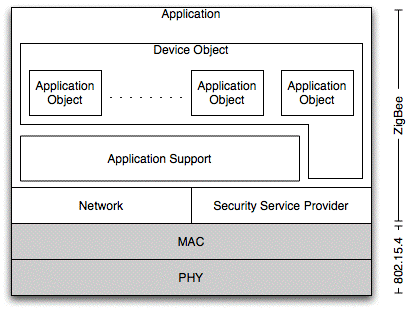
\includegraphics[width=15cm]{fig3.png}

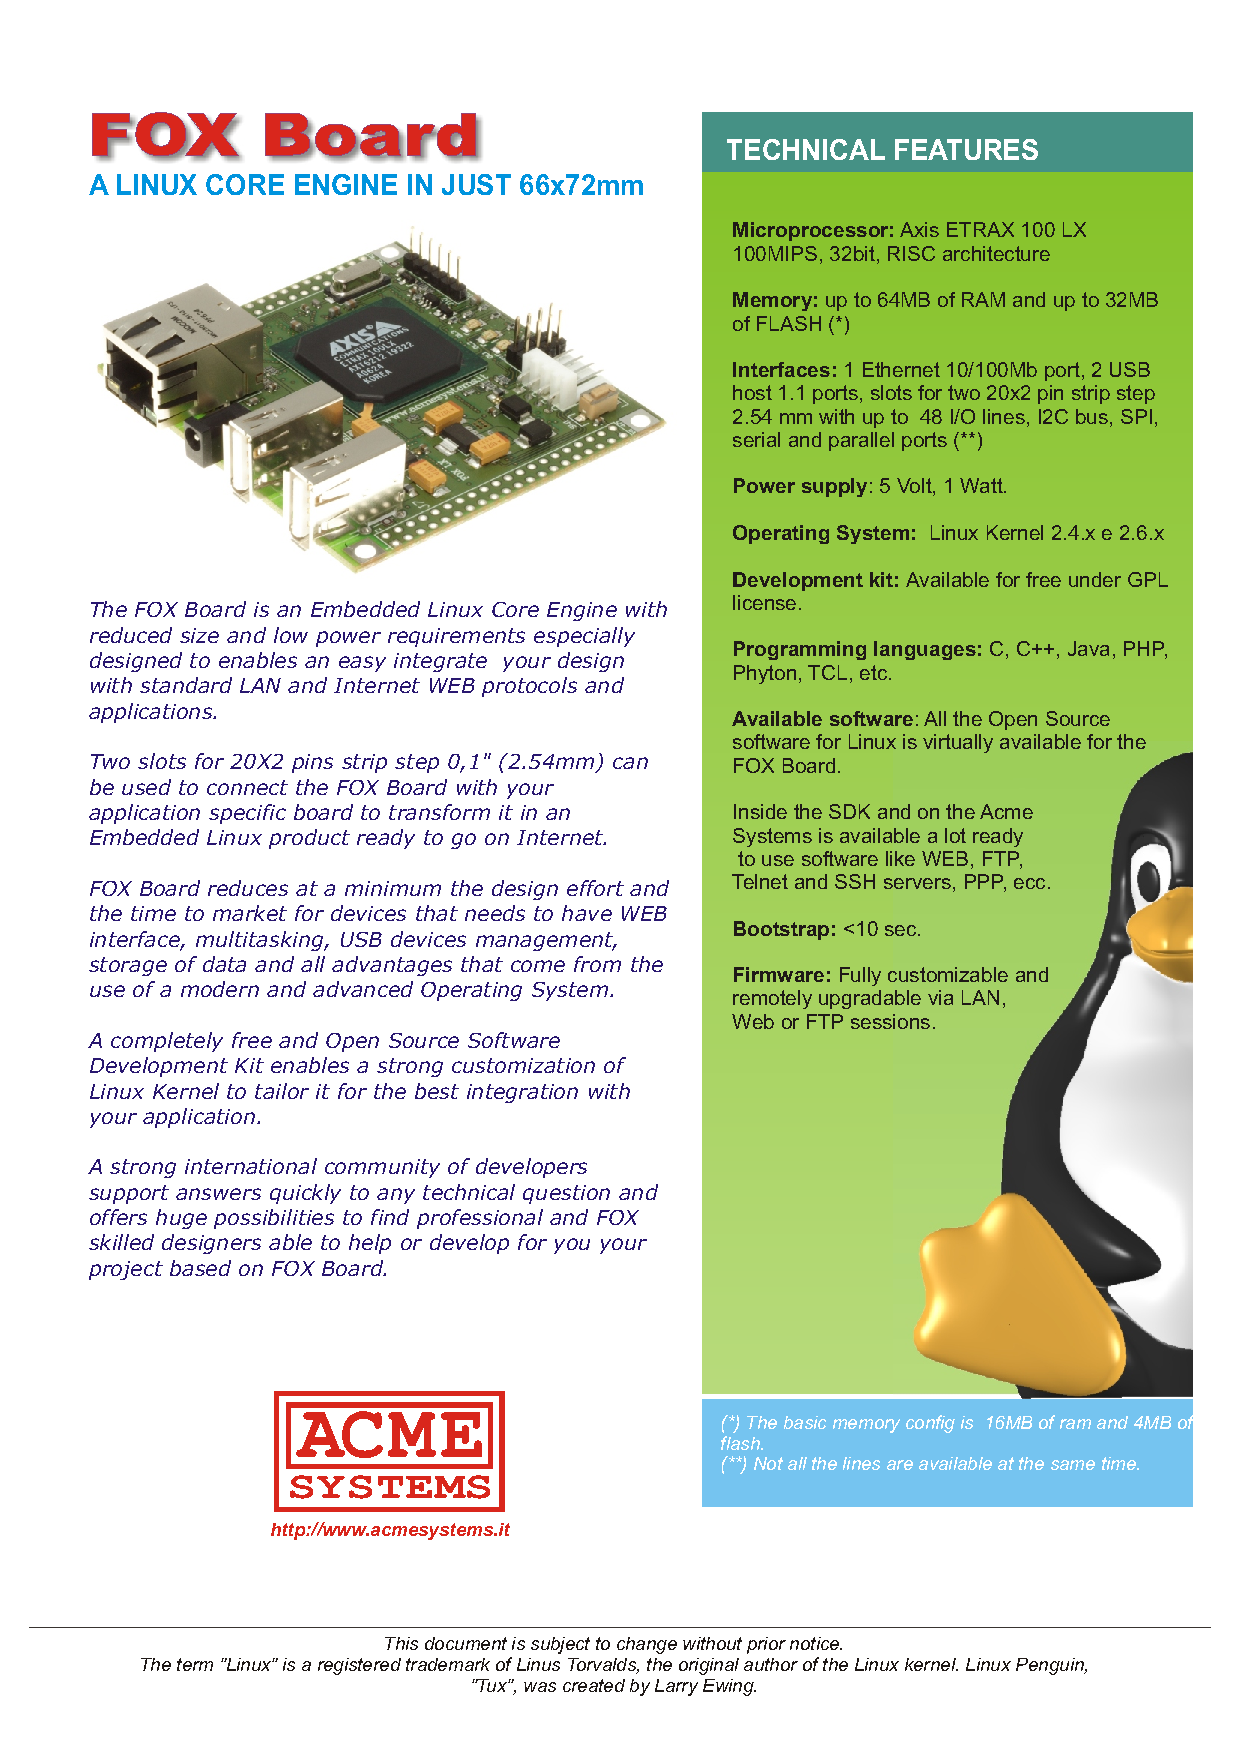
\includepdf{FoxDescription_en.pdf}
